\documentclass[border=10pt]{standalone}
\usepackage{tikz,amsmath}
\usetikzlibrary{shapes,calc,positioning}
\DeclareMathOperator{\IV}{IV}

\begin{document}
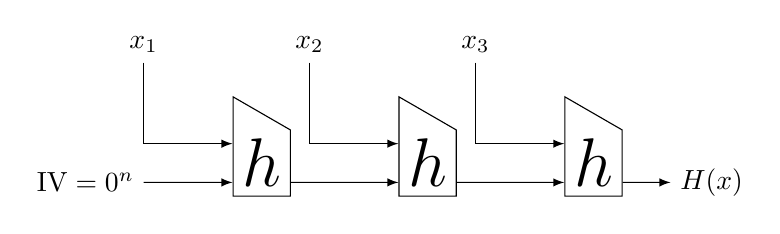
\begin{tikzpicture}[%
    on grid,
    node distance=1.5cm and 1.5cm,
    h/.style={%
        draw,
        trapezium,
        trapezium right angle=90,
        shape border rotate=270,
    }
]
\pgfmathsetlengthmacro{\inputsep}{0.7em};
    \node (x1) {$x_1$};
    \node[below=of x1, yshift=-\inputsep, anchor=east] (h0) {$\IV = 0^n$};
    \pgfmathsetmacro\last{3};
    \foreach \x in {1,...,\last}{%
        \pgfmathsetmacro\prev{\x-1};
        \ifnum \x > 1%
            \node[right=of x\prev] (x\x) {$x_\x$};
        \fi
        \node[h, below right=of x\x] (h\x) {\Huge $h$};
        \draw[-latex] (x\x) |- ($(h\x.west)+(0,\inputsep)$);
        \ifnum \x > 1
            \draw[-latex] ($(h\prev)-(0,\inputsep)$) -- ($(h\x.west)-(0,\inputsep)$);
        \fi
    }
    \draw[-latex] (h0) -- ($(h1.west)-(0,\inputsep)$);
    
    \node[right=of h\last, yshift=-\inputsep] (H) {$H(x)$};
    \draw[-latex] ($(h\last.east)-(0,\inputsep)$) -- (H);
\end{tikzpicture}
\end{document}
